El algoritmo toma como entrada un grafo no ponderado y la identificación del vértice de origen $s$. El grafo de entrada puede ser dirigido o no dirigido, no importa el algoritmo. 

El algoritmo se puede entender como un fuego que se propaga en el grafo: en el paso cero solo la fuente $s$ está en llamas. A cada paso, el fuego que arde en cada vértice se propaga a todos sus vecinos. En una iteración del algoritmo, el \emph{anillo de fuego} se expande en ancho en una unidad (de ahí el nombre del algoritmo).

Más precisamente, el algoritmo se puede establecer de la siguiente manera: Crear una cola $q$ que contendrá los vértices a procesar y un arreglo booleano $used[]$ que indica para cada vértice, si ha sido encendido (o visitado) o no. 

Inicialmente, adicione la fuente $s$ a la cola y establezca $used[s]=true$, y para todos los demás vértices v set $used[v]=false$. Luego, repita hasta que la cola esté vacía y, en cada iteración, extraiga un vértice desde el frente de la cola. Iterar a través de todos las aristas que salen de este vértice y si algunos de estos bordes van a vértices que aún no están encendidos, prende fuego y colócalos en la cola. 

Como resultado, cuando la cola está vacía, el \emph{anillo de fuego} contiene todos los vértices accesibles desde la fuente $s$, con cada vértice alcanzado de la manera más corta posible. También puede calcular las longitudes de las rutas más cortas (que solo requiere mantener una matriz de longitudes de ruta $d[]$), así como guardar información para restaurar todas estas rutas más cortas (para esto, es necesario mantener una matriz de $padres  p[]$, que almacena para cada vértice el vértice desde el que llegamos)

El siguiente ejemplo ilustra el funcionamiento del algoritmo BFS sobre un grafo de ejemplo. La secuencia de ilustraciones va de izquierda a derecha y de arriba hacia abajo. El algoritmo comienza por el nodo 0.

\begin{figure}[h]
	\centering 
	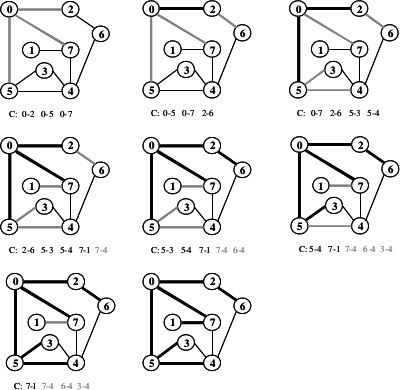
\includegraphics[scale=1.0]{img/bfs}
	\caption{Ejecucción del algoritmo BFS.}
	\label{contexto:figura1}
\end{figure}.

\subsection{BFS sobre tablero}
Una variante de este algoritmo es desarrollarlo sobre una matriz que en disimiles situaciones actua como un mapa de donde una celda se puede a unas de sus vecinas acorde a al concepto de vecinas que plantee el problema. Para este tipo de sistuaciones se trabaja con una matriz de visitados para saber cual celda de la matriz ha sido visitado y cual no. 

Además se utiliza una estructura para representar la celda de la matriz de la cual siempre en todas las ocasiones se almacena la fila y columna de dicha celda. El otro elemento en este tipo de situaciones son las llamadas matrices direccionales que ayudan de una forma más practica dada una celda hallar todas las celdas vecinas a esta dependiendo del problema. En la implementación del guía se pone un ejemplo de este caso muy peculiar pero super utilizado para resolver problemas.